\todo{Wichtige Begriffe erklären}

\subsection{Was bedeutet MOS-Technologie}
	\subsubsection{NMOS}
	\subsubsection{PMOS}
	\subsubsection{CMOS}
\subsection{MOS-Kondensatoren}
	\subsubsection{Grundaufbau}
	\subsubsection{Flachbandfall}
	\subsubsection{Anreicherung, Verarmung, Inversion}
\subsection{MOS-Transitoren}
	\subsubsection{Grundaufbau, neuere Entwicklungen usw.}
	
		%MOS Transistor
	\begin{center}
		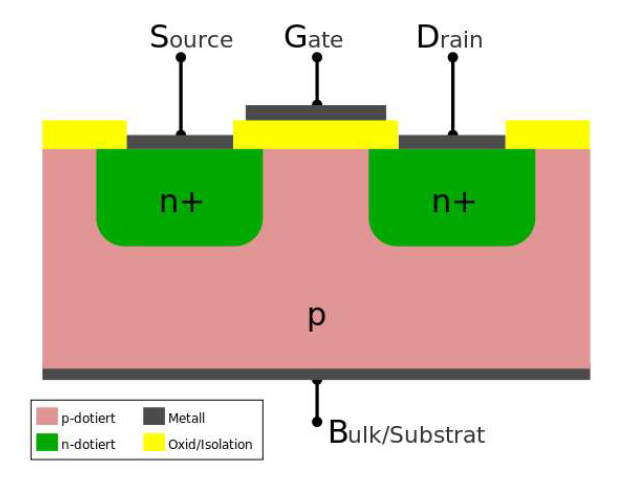
\includegraphics[width=0.7\linewidth]{Kapitel/Kap06/MOS_Transistor.png}
	\end{center}
		
	\subsubsection{Die vier Grundtypen}
	\subsubsection{Funktionsweise eines n-Kanal-Anreicherung-Transistoren}
	\subsubsection{Ausgangs- und Transferkennlinien}
\subsection{Anwendungen von MOS-Transistoren}
	\subsubsection{Vor- und Nachteile}
	\subsubsection{Funktionsprinzip eines CMOS-Inverter}


\todo{Fragen aus Own Clowd zuordnen}
\todo{Gruppenübungs-Inhalte ergänzen}